\documentclass[10pt,a4paper]{article}
\usepackage[utf8]{inputenc}
\usepackage{amsmath}
\usepackage{amsfonts}
\usepackage{amssymb}
\usepackage{graphicx}
\usepackage{parskip}
\usepackage{pdfpages}
\usepackage{tabularx}
\usepackage{pifont}
\usepackage{hyperref}
\usepackage{todonotes}
\usepackage{fancyvrb}
\usepackage{float}
\hypersetup{%
	pdfborder = {0 0 0}
}
\newcommand{\HRule}{\rule{\linewidth}{0.5mm}}


\newcommand{\cmark}{\ding{51}}%
\newcommand{\xmark}{\ding{55}}%

\begin{document}
	\begin{titlepage}
		\begin{center}
			
			% Upper part of the page. The '~' is needed because \\
			% only works if a paragraph has started.
			
			\textsc{\Large 02350 Windows Programming \\ 
				Autumn 2014 \\ 
				Technical University of Denmark}\\[1.5cm]
			
			\textsc{\Large Project Group 04}\\[0.5cm]
			
			% Title
			\HRule \\[0.4cm]
			{ \huge \bfseries A .Net Application for UML diagrams \\[0.4cm] }
			
			\HRule \\[1.5cm]
			
			% Author and supervisor
			\begin{center}
				\begin{minipage}{0.5\textwidth}
					\begin{flushleft} \large
						\emph{Authors:}\\
						Jonas \textsc{Pedersen} \\
						s123859 \\ ~ \\
						Peter \textsc{Gelsbo} \\
						s123397 \\ ~\\
						Kristian \textsc{Jagd} \\
						s123215
					\end{flushleft}
				\end{minipage}
			\end{center}
			
			
			
			\vfill
			
			% Bottom of the page
			{\large \today}
			
		\end{center}
	\end{titlepage}
	
	
	\pagenumbering{gobble}
	\thispagestyle{empty}
	
	
	\cleardoublepage
	
	
	
	\pagenumbering{arabic}
    \tableofcontents
	
	\newpage
	\section{Introduction}
The purpose of this document is to give an insight into how a diagram drawing
tool was created and how the choices and priorities formed the project. 

The aim for the project was to build a useable diagram tool for the Windows
platform using the \texttt{Windows Presentation Framework (WPF)}. Since the project is
created as a part of an only 5 ECTS points course, defining the scope is also an
important part of the task.

Since the product is not to be used by realworld customers, sometimes only the
most important aspects of a problem is solved, and tasks such as implementing a great varity of for
example relational arrows were not prioritized.

The overall structure of the report consists of the
\textit{Analysis} which outlines what exactly the application should do, to the
\textit{Design} that explains how it was achieved. In the \textit{Test} section
we validate that the solution indeed is solid and finally the project is wrapped
up in the \texttt{Discussion} and \texttt{Conclusion} section.

\subsection{Division of work}
All contributed evenly..

	\section{Analysis}
In the analysis the problem scope is defined by outlining the concept of the
application and lastly a more formal requirement list is used to prioritize the
different tasks.

\subsection{Application overview}
The application aims to make it easy for the users to create \textit{UML}
diagrams. To limit the scope, only the class diagram is required to be
functional, while the other types of diagrams should be easy to extend 
the program with. Therefore the most basic functionality includes creating
classes and filling those out with fields and methods. To create a proper
diagram these classes should also be arranged and connected with different
relations such as inheritance or composistion. Since it is an editor, auxiliary
editing functionaliy such as deleting classes or relations and undo/redo is
of great importance. 

A few more advanced features is also important to consider. Saving and loading a
diagram allows the user to create a diagram and then commit changes at a later
point.

A user could use the produced diagram in a presentation or in a report by
taking a screenshot of the application, but a better approch would be to export
an image which could be directly embedded. Therefore an export feature would be
a great addition to the program. 

Since the amount of functions for the program is limited, a user interface
optimized for quickly selection of the correct tool is important. This
includes hotkeys for the more proficient users. The original mockup from before
the development started can be seen in figure \ref{mockup}.

The UML class diagram has been chosen as the diagram type for this application, 
as this is the diagram type which the group members have the most proficiency with.

\begin{figure}[H]
\centering
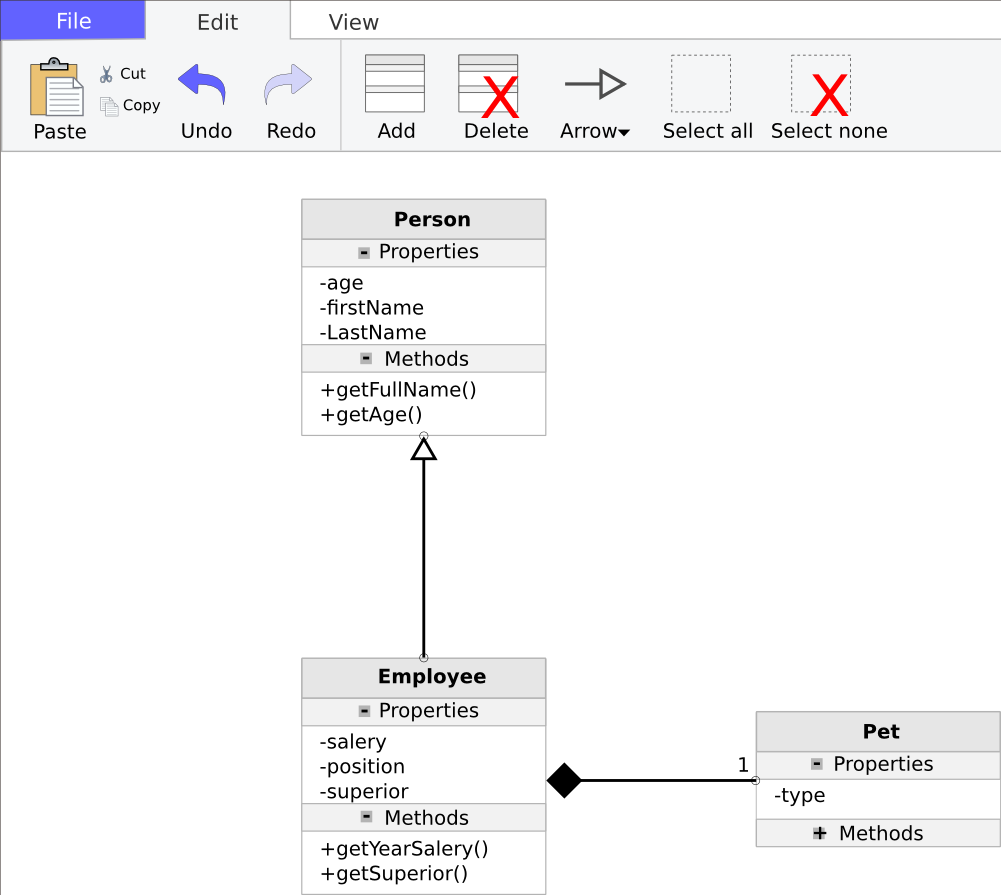
\includegraphics[width=\linewidth]{img/mockup}
\caption{Application mockup \label{mockup}}
\end{figure}

\subsection{Risks}
There are always the risk that certain elements of a program may end up taking
much longer than expected to implement.
This is especially true when none of the team-members have
used the tools before, as a lot of simple things has to be learned either by
trail-and-error or searching the internet for solutions. Therefore this is
tackled by using a priority list of the features, which secures that we get a
working version as early as possible, albeit with limited functionality. 

\newpage
\subsection{Requirements specification}
The specification is created using the \textit{MoSCoW} 
method\footnote{http://en.wikipedia.org/wiki/MoSCoW\_method}. Here, the 
requirements 
are divided in the following categories: \textit{Must}, \textit{should}, 
\textit{could} and \textit{won't}. This method can be seen as a combination of 
a requirements specification and an iteration plan, which helps the developers 
prioritize their work.

The application is a prototype and should not be considered as a final product 
but a basic concept ready for further development.

\begin{description}
	\item[Must have] \hfill \\
	\begin{enumerate}
		\item A graphical user interface supporting basic diagram editing 
		functionality
		\begin{itemize}
			\item Createing, editing and deleting classes
			\item Createing, editing and deleting relations
		\end{itemize}
		\item One diagram type
		\item DLL assembly containing the model for the diagram.
	\end{enumerate}
	\item[Should have] \hfill \\
	\begin{enumerate}
		\item Save/Open functionality
		\item Different relation types
		\item Undo/redo functionality
	\end{enumerate}
	\item[Could have] \hfill \\
	\begin{enumerate}
		\item Copy/cut/paste
		\item Export diagram as image
	\end{enumerate}
	\item[Won't have] \hfill \\
	\begin{enumerate}
		\item Multiple diagram types
		\item Advanced canvas functions
		\begin{itemize}
			\item Zoom
			\item Panning
		\end{itemize}
		\item Print funcionality
	\end{enumerate}
\end{description}






	\section{Design and implementation}

In this section the considerations for the
design will be discussed. This includes the overall design for the application
as well as the problems that the individual features posed. The section also
details how the proposed solutions were carried out and implemented in the
application.

\subsection{Overall design}
%Jonas
\subsubsection{Design patterns}

Mvvm, wpf, data bindings Model assembly

\subsubsection{Function list}
Based on the requirements and the definition of UML class 
diagrams\footnote{http://en.wikipedia.org/wiki/Class\_diagram} 
\footnote{http://www.digilife.be/quickreferences/qrc/uml quick reference 
card.pdf}, a function list is produced.

\begin{table}[H]
	\begin{tabular}{lll}
		\hline
		\textbf{Ribbon: File menu} 
		&                                                                       
		                     &
		                                                                        
		             \\ \hline
		New                        & \begin{tabular}[c]{@{}l@{}}Create new 
		project\\ Close/discard open project\end{tabular}    & 
		Ctrl+Shift+N                                                            
		            \\
		Open                       & Open existing 
		project                                                                 
		     &
		 
		Ctrl+O                                                                  
		            \\
		Save                       & Save current 
		project                                                                 
		      &
		 
		Ctrl+S                                                                  
		            \\
		Save As                    & Save current project as new 
		file                                                           & 
		Ctrl+Alt+S                                                              
		            \\
		Print                      & Print 
		diagram                                                                 
		             &
		 
		Ctrl+P                                                                  
		            \\
		Export                     & Export project to 
		PNG                                                                     
		 &
		 
		Ctrl+E                                                                  
		            \\
		 \hline
		&                                                                       
		                     
		&                                                                       
		              \\
		 \hline
		\textbf{Ribbon: Edit}      
		&                                                                       
		                     &
		                                                                        
		             \\ \hline
		Undo                       & Undo previous 
		actions                                                                 
		     &
		 
		Ctrl+Z                                                                  
		            \\
		Redo                       & Redo 
		actions                                                                 
		              &
		 
		Ctrl+Shift+Z                                                            
		            \\
		Paste                      & Paste class from 
		clipboard                                                               
		  &
		 
		Ctrl+V                                                                  
		            \\
		Cut                        & Cut 
		class                                                                   
		               &
		 
		Ctrl+X                                                                  
		            \\
		Copy                       & Copy selected 
		class                                                                   
		     &
		 
		Ctrl+C                                                                  
		            \\
		New Class                  & Add 
		class                                                                   
		               &
		 
		Ctrl+N                                                                  
		            \\
		Delete Class               & Delete selected 
		class                                                                   
		   &
		 
		Delete                                                                  
		            \\
		Relations                  & \begin{tabular}[c]{@{}l@{}}Add relation 
		between classes\\ (enter add mode)\end{tabular}    
		&                                                                       
		              \\
		Delete relation            & \begin{tabular}[c]{@{}l@{}}Delete 
		relation\\ (show circle, enter delete mode)\end{tabular} 
		&                                                                       
		              \\
		 \hline
		&                                                                       
		                     
		&                                                                       
		              \\
		 \hline
		\textbf{Canvas functions}  
		&                                                                       
		                     &
		                                                                        
		             \\ \hline
		Select class               
		&                                                                       
		                     &
		 Click on 
		class                                                                   
		   \\
		Drag class                 
		&                                                                       
		                     &
		 Drag class with 
		mouse                                                               \\
		Add relation               & (during add relation 
		mode)                                                                 & 
		\begin{tabular}[c]{@{}l@{}}Click on class "from"\\ Click on class 
		"to"\end{tabular} \\
		Delete relation            & (during delete relation 
		mode)                                                              & 
		\begin{tabular}[c]{@{}l@{}}Click on relation\\ 
		(circle)\end{tabular}                \\
		Change class name          
		&                                                                       
		                     &
		 Click on text 
		field                                                                 \\
		Add field / method         
		&                                                                       
		                     &
		 Click 
		+                                                                       
		      \\
		Remove field / method      
		&                                                                       
		                     &
		 Click 
		X                                                                       
		      \\
		Edit field/method text     
		&                                                                       
		                     &
		 Click on text 
		field                                                                 \\
		Edit relation text         
		&                                                                       
		                     &
		 Click on text 
		field                                                                 \\
		Edit multiplicity text     
		&                                                                       
		                     &
		 Click on text 
		field                                                                 \\
		 \hline
	\end{tabular}
\end{table}



\subsection{Graphichal User interface}

\subsubsection{Design}

Even though that
user interface design was not a main scope of the project, some thought is
required as it greatly impacts the user experience. 

The overall decision to make it wether to whether to use an existing design
framework, or to create a whole new layout with toolbars, menues etc. Since it
is not in the scope of the project and the benefit would be minimal it was
decided to go with an already tested and know interface. 

The traditional Windows application is defined by its layered menus and toobars,
which execls at more complicated programs where submenus are essential.

The other viable alternative is the
\textit{Ribbon}\footnote{http://msdn.microsoft.com/en-us/library/windows/desktop/dd316910(v=vs.85).aspx}
framework which is know for its big toolbar with the most used functions ready
for use.

Based on the original program mockup as previously seen in figure \ref{mockup},
it was clear that all the menu items could be in such a bar that the Ribbon
interface offers without creating additional layers.

It also seemed a good fit for a graphical editing tool, as the Ribbon interface
has an emphasis on having a graphical display for each action. This makes the
tool a lot easier to use for new users, as for example a relation could be
accompanied by a graphical representation showing exactly how the relation will
look like.

\subsubsection{Implementation} 
The \textit{GUI} was created with \texttt{XAML} and the standard windows
\textit{Ribbon} API. \texttt{XAML} supports defining all the graphical elements,
but also data bindings and user events.


Menu, ribbon, user controls etc.

\subsubsection{Implementation}
Menu, ribbon, user controls etc.


\subsection{Application}
In this part the application part of the program is discussed.

\subsubsection{Klasses and relations}
%Jonas
The \texttt{Klass} and \texttt{Relation} classes are the backbone of the model.
So they were put in their own \texttt{dll}. This ensures reusability, and makes
the program more flexible, in that it does not consist of 1 giant exe file.

\paragraph{Klass}
The \texttt{Klass} class is the representation of a class in any object oriented
language. The class contains almost all the info a class should have. Some of
the missing stuff is interfaces and abstract classes, but these can be added in
future iterations.

The class also contains some of the info needed to render it properly, such as
an $(x, y)$ coordinate as well as such things as height, width, and some color
properties. Some of this probably belongs in a viewmodel class but we found it
easier to just implement it directly in this class instead.

The consequence of having viewmodel properties in the model, was that
\texttt{Klass} also had to have a list of all the relations that was hooked up
to it. This was to be able to notify any relation whenever a \texttt{Klass} is
moved in the GUI. 

What became easier from having the viewmodel properties in the model, was the
serialization, and how to handle the relation between \texttt{Klass} and
\texttt{Relation}. Having a relation between the 2 models, and 2 viewmodels
would make it hard to maintain the right state.

\paragraph{Relation}
The \texttt{Relation} class is used to represent the relation in a UML diagram.
This class has to be flexible to allow for many different types of relations,
such as inheritance, reference, composition, etc. The class uses an enum to know
which type of relation it is. This eliminates the need to create a new subclass
every time a new type of relation is introduced.

\subsubsection{Saving \& loading}
The save and open functionality is based on the serialization process. Objects
can be serialized to a sequence of bytes either as binary data or in an XML
structure. The serialized data can be stored in a file, and loaded into the
application later by deserializing the objects.

For this project, two solutions were considered. Using the functionality in the
\texttt{System.Runtime.Serialization} namespace, or using the XmlSerializer
class from the \texttt{System.Xml.Serialization} namespace. The Runtime
Serialization allows us to store the serialized objects as binary data or
formatted as SOAP data.

The three options all have their advantages and disadvantages. We have chosen
runtime serialization with binary formatting, based on what we found as
described in the following sections.

\paragraph{XML Serializer}

The 
\texttt{XmlSerializer}\footnote{http://msdn.microsoft.com/en-us/library/system.xml.serialization.xmlserializer}
 class provides easy to use
functionality to serialize and deserialize simple objects to an XML format. It
is possible to define which objects are serializable, and which field of objects
that should be serialized, and which should not.

However, the XmlSerializer class, does not support references to objects. This
means, that every time the serializer meets a serializable object, the object
will be serialized - even though it may already have done so. This does not
allow for cyclic references, which we have in our program. In our case, a Klass
object references a list of Relations, which in turn references a To and From
Klass.

If we were to use the XmlSerializer class, we would have to change the structure
of our program.

\paragraph{Runtime serialization}

The classes in the runtime serialization
namespace supports references to objects. When the serializer meets an object,
which has already been serialized, the object is referenced and not
re-serialized.

The behaviour is defined by the interface 
\texttt{ISerializable}\footnote{http://msdn.microsoft.com/en-us/library/system.runtime.serialization.iserializable}
 which contains the method \texttt{GetObjectData}. This method allows us to 
define exactly which fields of an object that should be serialized and how to 
serialize them. To deserialize an object, a special deserialization constructor 
must be defined, which tells the serializer how to interpret the saved data.

The runtime serialization allows for two types of formatting: Binary and SOAP.

\textbf{Binary formatting}\\
Binary formatting serializes the objects to a
sequence of bytes, which is unreadable to humans. It works, but it has the
disadvantage, that it can be hard to verify, that the serializer does what it is
meant to do.

\textbf{SOAP formatting}\\
SOAP is a protocol used to exchange information, and
is often used in web services which provide data to other applications through
an API. The resulting data when using SOAP formatting is an XML structure,
similar to the structur of the XmlSerializer and iis more friendly to human
interpretation than its binary counterpart.

However, for some reason, the SOAP formatter attempted to serialize objects from
our MVVM libray, even though it was not told to, which made the serialization
fail.

\paragraph{Save \& open dialogs}
To allow the user to save and open diagram files, the standard save- and open 
file dialog boxes are utilized. This functionality allows us to define which 
files the user should see; in our case \emph{.dia} files.

\begin{figure}[H]
	\centering
	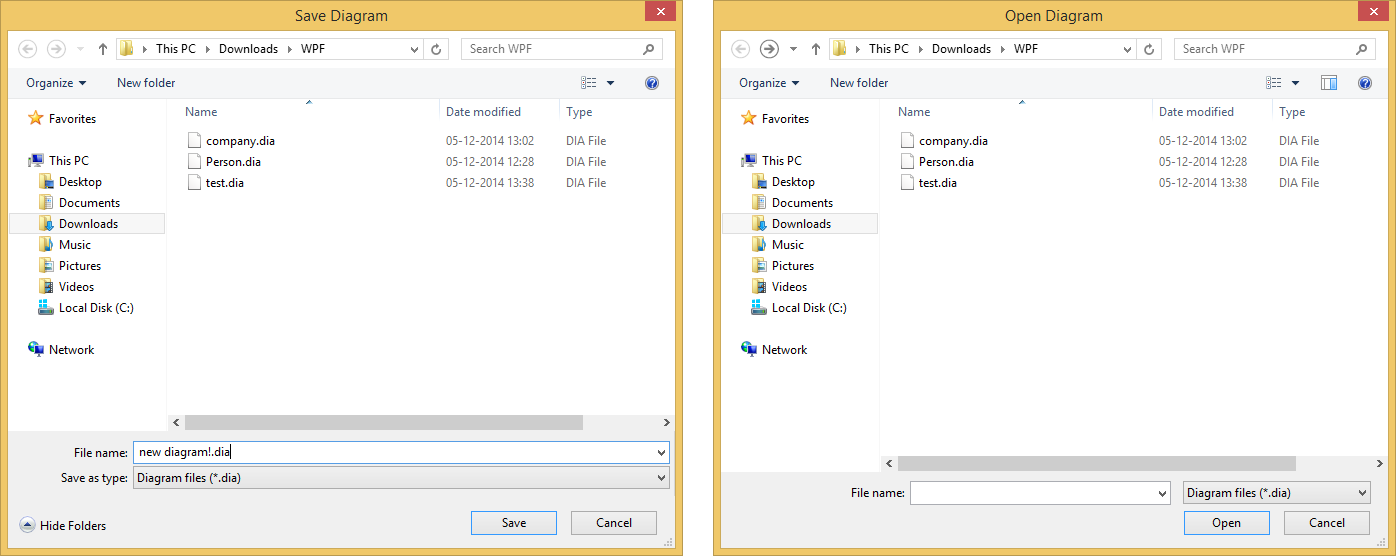
\includegraphics[width=\linewidth]{img/save_open.png}
	\caption{Save and open dialog boxes \label{saveopen}}
\end{figure}

\subsubsection{Using threads}
Serialization, deserialization and reading/writing
to files are processes that might take some time for the computer to execute.
Thus, threads can be used to improve the user experience by preventing the
window from “freezing” while these processes are going on. Typically, the
diagrams made in this program are relatively small and simple, and the user may
not notice anything when saving and opening without threads. However, the
difference may be noticeable if the users hard drive is really slow, or the
diagram is really big.

In our case, the saving process is handled by a thread, which allows the user to
continue working while the objects are saved in the background. Opening files
are not executed in a thread, since the user should wait for everything to be
loaded anyway. It could easily be implemented, but the save functionality
exemplifies the process quite well.


\subsubsection{Undo / Redo}
%Peter
All commands supporting the undo/redo functionality implments the
\texttt{IUndoRedoCommand} interface, which extends \texttt{ICommand}. The 
singleton class
\texttt{UndoRedoController} handles the undo- and redo-stacks, which keep track 
of the
previous states of the application. All UndoRedoCommands are executed through
the AddAndExecute methods, of this class.

The applications enables undo/redo functionality on the following actions:


\begin{itemize}
	\item New class
	\item Delete class
	\item Add relation
	\item Delete relation
	\item Cut
	\item Paste
	\item Move class
\end{itemize}


\subsubsection{Copy, cut \& paste}

A simple clipboard is implemented in the
application to allow copying, cutting and pasting classes. When pasting a class
from the clipboard, the class and its content (fields and methods) are copied,
but not its relations. This behaviour is intended, as we believe that this is
the typical use case for copy/paste.

The clipboard functionality utilizes the existing commands for deleting and
creating new classes, hence, it supports the undo/redo functionality of
those.

This solution only supports copy paste of class objects. If it made sense, this 
could be extended to support additional objects. The implementation does not 
overwrite the built in clipboard of Windows. Thus, the user can still 
copy/paste text from and to text fields within the application.

\subsubsection{Image export}

To make it easier for the users to use the created diagram, an image export tool
was implemented. Only support for \textit{png} was implemented as it it
the most suited filetype for this kind of graphics. An important thing to consider
is how to ensure that only the relevant part of the canvas it exported, so
the users does't have to crop the image later.

\texttt{Export} was implemented in the \texttt{MainViewModel}, by creating a
\texttt{RelayCommand} that takes the canvas as argument.
The \texttt{Export} method then finds all the  descendants bounds, which is 
the minimum area that ensures that all relevant elements are exported. The
default renderer however always renders from $(0,0)$, so an auxiliary method to
cancel this offset was used. The standard Windows Save dialog was used toi
select the image path.


	\section{Tests}

The tests made for this project, is primarily done with unit
tests. The program ui has been tested by hand.

\subsection{Unit Test 1 - Add new class}

The user may want to add a new class to the model. By pressing the button, it is
possible to observe that a new class indeed appears. The test tests to see if a
new \texttt{Klass} instance has been added to the \texttt{MainViewModel}'s
collection.

\subsection{Unit Test 2 - Remove class}

The user may also want to remove a class from the diagram. In this case, it is
necessary to first select a class, and then call remove.

It is then asserted that the class is removed from the \texttt{Klasses}
collection.

It is also tested for the case when no class is selected. In this case, nothing
should happen.

Instead of letting nothing happen, it would be possible to throw an exception.
This would also make it possible to warn the user if necessary.

\subsection{Unit Test 3 - Copy/Paste class}

This test is to make sure that the copy pasted class is added to the viewmodel,
and that it is a deep copy.

This functionality also relies on a selected class, so it is also tested that
nothing happens when no class is selected.

The user may also want to paste a class multiple times. These extra copies does
also have to be deep copies, and the user should be able to paste multiple times
without having to reselect a class.


\subsection{Unit Test 4 - Setting a relation}

The user should be able to add a relation between 2 models. It is crucible in
the model, that a relation has a reference to each class, and that each class has
a reference to each relation.

The test makes sure that it happens.

\subsection{Unit Test 5 - Unsetting a relation}

It is possible to remove a relation. Since this affects the state of the program
multiple places when set, they all have to be reverted when unset.


\subsection{Code coverage}

\begin{figure}
\centering
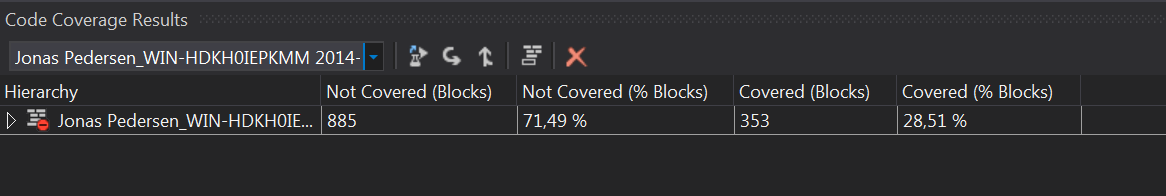
\includegraphics[width=0.85\linewidth]{img/coverage}
\caption{Screenshot of the Visual Studio code coverage tools result.}
\end{figure}

The tests cover approximately $30\%$ of all the code. Achieving $100\%$ would
likely take as long time as making the project itself, so only the most
important, and most likely to break stuff, was tested.

It would also be hard to test the GUI part of the program, and since e.g.
AddRelation relies on mouse clicks, it would be hard to make unit test for.

	\section{Discussion}
In this section the resulting product is discussed including what gave us trouble and
which features and changes could be relevant in the future if further
development was needed.

\subsection{Problems and bugs}
Input / focus
Linecaps / VS / git

\subsection{Futher development}
Easy to add relations / other diagram types
Better canvas zoom / panning
copy paste text
	\section{Conclusion}

This document has explained how a diagram tool for the windows platform was
created with \texttt{WPF}. 

The program was built around the \textit{Model View ViewModel} design pattern
which enabled us to keep the business and presentation layer separated. The
business layer was implemented as a \texttt{model} assembly, and the
presentation layer was written in \texttt{XAML}. By using data bindings the two
were connected in a powerful way. 

During the project we had to set a scope that fit the available time. Since none
of the team-members had worked with the \texttt{WPF} framework previously, a lot
of time went towards learning it in the beginning. In this period mostly basic
features such as the \texttt{Ribbon} toolbar and the class model and view was
created. When the team got more proficient with tools, more advanced features
were added, such as a flexible way to add relations, saving and loading diagrams
and exporting to png. 

In the end the product turned out to be a rather complete prototype as all of
the basic functionality was implemented and even a few of the advanced features
was introduced. The program lays a good foundation for further development, as
it would be easy to extend with additional diagram types, canvas controls, etc.

\end{document}
